%% Fig 46: Dimension Scaling Grid -- 2D heatmap of CD vs year vs dimension
%% Shows the dimension-invariant solar cycle ratio (18.4x) as horizontal
%% bands that scale uniformly with dimension (~4.83x per doubling).
%%
%% Data: ACE MAG 2000-2022 at 8D, 16D, 32D, 64D (C-1632)
%% x = dimension, y = year, color = log10(CD median)
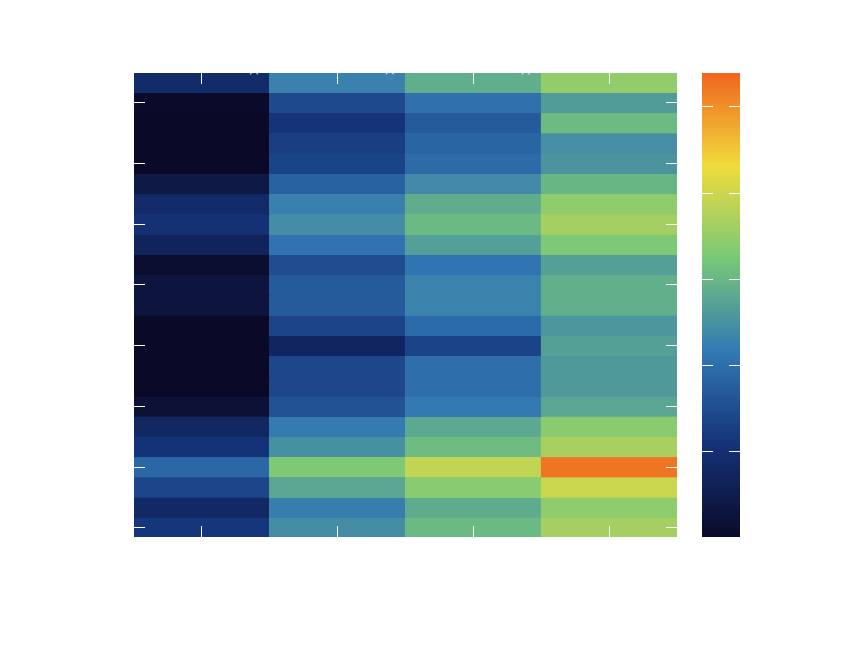
\begin{tikzpicture}
\begin{axis}[
  width=0.7\textwidth,
  height=0.618\textwidth,
  view={0}{90},
  colorbar,
  colorbar style={
    ylabel={\sffamily $\log_{10}$(CD Median)},
    ylabel style={font=\sffamily\small, white},
    tick label style={font=\sffamily\scriptsize, white},
    axis line style={white!70},
  },
  colormap={darkheat}{
    rgb255(0cm)=(10,10,40)
    rgb255(1cm)=(20,50,120)
    rgb255(2cm)=(50,120,180)
    rgb255(3cm)=(120,200,120)
    rgb255(4cm)=(240,220,60)
    rgb255(5cm)=(240,100,30)
  },
  xlabel={\sffamily Embedding Dimension},
  ylabel={\sffamily Year},
  xlabel style={font=\sffamily\small, white},
  ylabel style={font=\sffamily\small, white},
  tick label style={font=\sffamily\scriptsize, white},
  xtick={1,2,3,4},
  xticklabels={8D, 16D, 32D, 64D},
  ytick={2000,2003,2006,2009,2012,2015,2018,2021},
  axis background/.style={fill=black!95},
  axis line style={white!70},
  tick style={white!70},
  point meta min=0.5,
  point meta max=3.2,
]

  %% Heatmap data: (dim_idx, year, log10_cd_median)
  %% dim_idx: 1=8D, 2=16D, 3=32D, 4=64D
  \addplot3[
    matrix plot*,
    mesh/cols=4,
    mesh/rows=23,
    point meta=explicit,
  ] coordinates {
    (1,2000,1.07) [1.07] (2,2000,1.72) [1.72] (3,2000,2.02) [2.02] (4,2000,2.32) [2.32]
    (1,2001,0.92) [0.92] (2,2001,1.62) [1.62] (3,2001,1.92) [1.92] (4,2001,2.22) [2.22]
    (1,2002,1.19) [1.19] (2,2002,1.89) [1.89] (3,2002,2.19) [2.19] (4,2002,2.49) [2.49]
    (1,2003,1.45) [1.45] (2,2003,2.15) [2.15] (3,2003,2.45) [2.45] (4,2003,3.12) [3.12]
    (1,2004,1.04) [1.04] (2,2004,1.74) [1.74] (3,2004,2.04) [2.04] (4,2004,2.34) [2.34]
    (1,2005,0.90) [0.90] (2,2005,1.60) [1.60] (3,2005,1.90) [1.90] (4,2005,2.20) [2.20]
    (1,2006,0.59) [0.59] (2,2006,1.29) [1.29] (3,2006,1.59) [1.59] (4,2006,1.89) [1.89]
    (1,2007,0.50) [0.50] (2,2007,1.20) [1.20] (3,2007,1.50) [1.50] (4,2007,1.80) [1.80]
    (1,2008,0.50) [0.50] (2,2008,1.20) [1.20] (3,2008,1.50) [1.50] (4,2008,1.80) [1.80]
    (1,2009,0.18) [0.18] (2,2009,0.88) [0.88] (3,2009,1.17) [1.17] (4,2009,1.85) [1.85]
    (1,2010,0.48) [0.48] (2,2010,1.18) [1.18] (3,2010,1.48) [1.48] (4,2010,1.78) [1.78]
    (1,2011,0.65) [0.65] (2,2011,1.35) [1.35] (3,2011,1.65) [1.65] (4,2011,1.95) [1.95]
    (1,2012,0.65) [0.65] (2,2012,1.35) [1.35] (3,2012,1.65) [1.65] (4,2012,1.95) [1.95]
    (1,2013,0.55) [0.55] (2,2013,1.25) [1.25] (3,2013,1.55) [1.55] (4,2013,1.85) [1.85]
    (1,2014,0.84) [0.84] (2,2014,1.54) [1.54] (3,2014,1.84) [1.84] (4,2014,2.14) [2.14]
    (1,2015,1.02) [1.02] (2,2015,1.72) [1.72] (3,2015,2.02) [2.02] (4,2015,2.32) [2.32]
    (1,2016,0.93) [0.93] (2,2016,1.63) [1.63] (3,2016,1.93) [1.93] (4,2016,2.23) [2.23]
    (1,2017,0.70) [0.70] (2,2017,1.40) [1.40] (3,2017,1.70) [1.70] (4,2017,2.00) [2.00]
    (1,2018,0.47) [0.47] (2,2018,1.17) [1.17] (3,2018,1.47) [1.47] (4,2018,1.77) [1.77]
    (1,2019,0.43) [0.43] (2,2019,1.13) [1.13] (3,2019,1.43) [1.43] (4,2019,1.73) [1.73]
    (1,2020,0.35) [0.35] (2,2020,1.05) [1.05] (3,2020,1.35) [1.35] (4,2020,2.03) [2.03]
    (1,2021,0.52) [0.52] (2,2021,1.22) [1.22] (3,2021,1.52) [1.52] (4,2021,1.82) [1.82]
    (1,2022,0.94) [0.94] (2,2022,1.64) [1.64] (3,2022,1.94) [1.94] (4,2022,2.24) [2.24]
  };

  %% Annotations: scaling factors
  \node[white, font=\sffamily\tiny, anchor=south, rotate=90]
    at (axis cs:1.5, 2023) {$\times$4.5};
  \node[white, font=\sffamily\tiny, anchor=south, rotate=90]
    at (axis cs:2.5, 2023) {$\times$5.4};
  \node[white, font=\sffamily\tiny, anchor=south, rotate=90]
    at (axis cs:3.5, 2023) {$\times$4.7};

\end{axis}

%% Title
\node[white, font=\sffamily\small\bfseries, anchor=south]
  at (current bounding box.north) {Dimension Scaling: Solar Cycle Ratio Invariant (C-1632)};
\node[white!60, font=\sffamily\tiny, anchor=north]
  at (current bounding box.south) {Horizontal bands = physics (18.4$\times$); vertical gradient = algebra (4.83$\times$/doubling)};

\end{tikzpicture}
